\documentclass[10pt,twoside]{article}
\usepackage[pdftex]{graphicx}
\usepackage[small,bf,sf,textfont={small,sf,bf}]{caption}
\usepackage{subfig}
\usepackage{amsmath}
\usepackage{fancyheadings}
\usepackage{SPE}
\usepackage{pslatex}
\usepackage{color}
\usepackage{graphicx}
\usepackage{graphics}
\graphicspath{{images/}}
\usepackage[round]{natbib}

\setlength{\textheight}{9.4in}

\begin{document}

\pagestyle{fancy}

\lhead
[\small \sffamily \thepage]{\small \sffamily SPE-195036-MS}
\rhead[\small \sffamily SPE-195036-MS]{\small\sffamily \thepage}

\rfoot[]{}
\cfoot[]{}
\lfoot[]{}

\setlength{\columnseprule}{0pt}

\newcommand{\trp}{^{\scriptsize \text{T}}}
\newcommand{\itp}{^{\scriptsize -\text{T}}}
\newcommand{\sqrtp}{^{\scriptsize \text{T/2}}}
\newcommand{\isqrtp}{^{\scriptsize -\text{T/2}}}
\newcommand{\inv}{^{\scriptsize -1}}
\newcommand{\sqr}{^{\scriptsize \text{1/2}}}
\newcommand{\invsqr}{^{\scriptsize -\text{1/2}}}

\newcommand{\TCR}[1]{\textcolor{red}{{#1}}}
\newcommand{\TCB}[1]{\textcolor{blue}{{#1}}}
\newcommand{\TCM}[1]{\textcolor{magenta}{{#1}}}

\thispagestyle{empty}
\vspace*{-1.0in}

\begin{figure}[!ht]
\flushright

\includegraphics[width=0.23\textwidth]{./SPEInt}
\setlength{\abovecaptionskip}{-10pt}
\end{figure}


{\noindent \sffamily \Large SPE-195036-MS}

\vspace*{32pt}

{\noindent \sffamily \Large {Beyond Steel Casing: Detecting Zonal Isolation in the Borehole Environment}}


{\noindent \sffamily T. Eltsov and T.W. Patzek}

        \noindent\textit{Ali I. Al-Naimi Petroleum Engineering Research Center, King Abdullah University of Science and Technology}\newline

\bigskip

\noindent \parbox[t]{7.5in}{ \scriptsize \sffamily \noindent
Copyright 2019, Society of Petroleum Engineers

\medskip

\noindent This paper was prepared for presentation at the SPE Middle East Oil and Gas Show and Conference, Bahrain, 18 - 21 March 2019.

\medskip

\noindent This paper was selected for presentation by an SPE program committee following review of information contained in an abstract submitted by the author(s). Contents of the paper have not been reviewed by the Society of Petroleum Engineers and are subject to correction by the author(s). The material does not necessarily reflect any position of the Society of Petroleum Engineers, its officers, or members. Electronic reproduction, distribution, or storage of any part of this paper without the written consent of the Society of Petroleum Engineers is prohibited. Permission to reproduce in print is restricted to an abstract of not more than 300 words; illustrations may not be copied. The abstract must contain conspicuous acknowledgment of SPE copyright.

\noindent \hrulefill}

\section*{Abstract}
\label{Sec:Abstract}

{Electrically resistive composite casing materials are being introduced to the oil \& gas industry. Resistive casing enables electromagnetic logging for exploration and reservoir monitoring, but it requires development of new logging methods.} Here we present a technique for the detection of integrity of magnetic cement behind resistive casing. We demonstrate that an optimized induction logging tool can detect small changes in the magnetic permeability of cement through a non-conductive casing in a vertical (or horizontal) well. We can determine both integrity and solidification state of the cement filling annulus behind casing.  Changes in magnetic permeability influence mostly the real part of the vertical component of magnetic field. The signal amplitude is more sensitive to a change of magnetic properties of the cement, rather than the signal phase. Our simulations show that optimum separation between the transmitter and receiver coils ranges from 0.25 to 0.6 meters, and the most suitable magnetic field frequencies vary from 0.1 to 10 kHz. {A high-frequency induction probe operating at 200 MHz can measure the degree of solidification of cement.} The proposed method can detect borehole cracks filled with cement, incomplete lift of cement, casing eccentricity and other borehole inhomogeneities.

\section{Introduction}
\label{Sec:Intro}

Evaluation of cement integrity is of primary importance to the industry. Poor cementation can lead to costly accidents and a serious damage to the environment. According to the \citet{Bp2010} report, one of the reasons for the Macondo well blowout on 20 April, 2010, was poor zonal isolation with a foam cement. Thus, better cement placement and better evaluation of cement quality must both be considered. Magnetic particles are used in different applications. They allow to solve various tasks remotely. In medicine, they are used for drug delivery system, cancer diagnosis or bio separation \citep{Ito2005}. In the oil industry, they are used for hydraulic fracture evaluation, EOR and other applications \citep{Guo2015}. Magnetorheological approach can be used to inject uniformly cement slurry into annular space between the casing and borehole wall. Magnetic cement slurry can be displaced into the regions where it would not otherwise flow when pumped conventionally \citep{Nair2013}. Magnetic properties of cement change with time, because of heating and aging. Electrical properties of the cement-based magnetorheological fluid differ from those of common cements. Presence of conductive particles increases magnetic permeability of cement \citep{Nair2016} and, because of proximity of the cement-filled annulus to the casing, one can use the magnetic susceptibility logging method to determine cement quality. It is necessary to estimate magnitude of the useful signal and establish appropriate measurement methods. This leads to an assessment of accuracy of the sensors or magnetometers that should be installed in the magnetic cement sensing tool. A thorough analysis of available sensors and frequency ranges helped us compile Fig.~\ref{sensors_range}. Measurement of electromagnetic fields for geophysical purposes covers a range wider than in most of other fields. For example, when performing cross-well EM exploration, the noise level has been estimated as $0.5 \cdot 10^{-5}$ nT,~\citep{Marsala2015}. The magnitudes of magnetic fields used in cardiac or brain medical research are also very small and require precise and expensive equipment. We do not need such high accuracy for assessing quality of magnetic cement; flux-gate magnetometers, Hall-effect sensors, or solenoid type sensors are quite sufficient.

\begin{figure}[ht!]
\centering
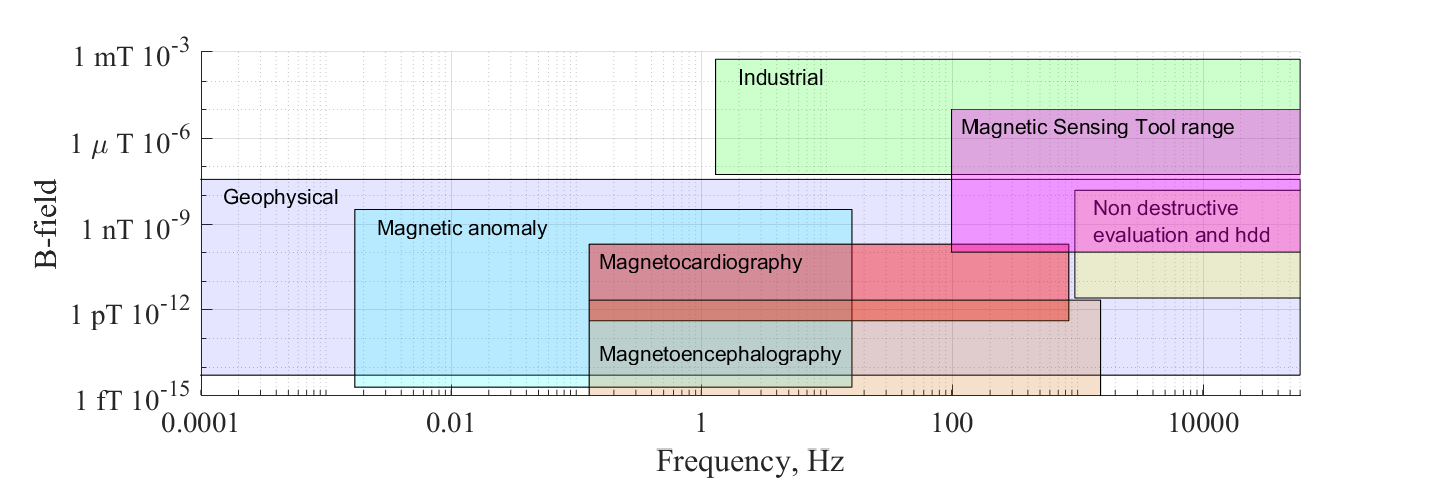
\includegraphics[scale=0.85]{sensors_range.eps}
\vskip2pt
\caption{{Magnetic field ranges and frequencies used in different disciplines, compiled after \citet{Ripka2001}. The range of B-field magnitude and frequency used in the numerical experiments discussed in this paper is marked with magenta.}}
\label{sensors_range}
\end{figure}

Measuring electrical properties through casing was a great challenge in the second part of last century. The complex effects of casing were captured long ago and solutions were found \citep{Alpin1939, Stewart1949}, providing two methods of logging in cased wells. Because of the high conductivity of steel casing relative to surrounding formation, the expected measurements are to be made in the nanovolt range \citep{Aulia2001}. Technical and computing capabilities of the industry in 1940s were insufficient for such precise measurements. \citet{Kaufman1990} has developed a theory of measuring formation resistivity in cased borehole with sufficient accuracy for practical applications. This theory has been implemented, and nowadays Schlumberger provides the formation resistivity log in cased borehole, called CHFR \citep{Aulia2001, Gyllensten2001}. To be of sufficient quality, this log takes about 12 hours to run, with each measurement consuming about 2 minutes. There are theoretical preconditions for logging through casing on the basis of magneto-acoustic effects \citep{Dorovsky2013,Dorovsky2017}. It is proposed to estimate electrical properties from an acoustic signal generated by a sensor responding to acoustic waves at a metal surface in communication with an earth formation. The metal surface is exposed to a constant magnetic field normal to it and a harmonic magnetic field of variable frequency along the surface. Further development of this method requires additional laboratory experiments.


Existing methods of estimating electrical properties behind casing are not suitable for assessing the electrical properties of cement. These methods evaluate the integral electrical formation properties at a distance away from the casing or are currently underdeveloped. In this paper, we propose a tool to measure and control integrity of the weakly magnetic cements behind nonconductive fiberglass casing. The objective is to verify cement quality in a borehole environment by computing the tool parameters - distance between coils and operating frequencies.  Borehole environment is magnetized  by a low frequency induction tool. Measurements can be made with a set of coils or sensors. Alternating magnetic field provides necessary noise immunity of logging and excludes the influence of the geomagnetic field \citep{Saraev2004}.  Significant work has been devoted to studying the influence of electrical properties of borehole media on the electromagnetic logging signals, such as dielectric permeability and its distribution \citep{Yeltsov2016}, or change of electrical resistivity of the invaded zone \citep{Eltsov2011}. Effect of magnetic permeability on inductive response has been studied for metal detector applications \citep{Das2006} and logging applications \citep{Barber1995, Hu2009}. However, cement detection and measurement of cement integrity have not been studied sufficiently for weakly magnetic cements. Here we focus on detecting small changes in the magnetic permeability of cement-filled annulus behind a non-conductive casing.


\section{Methods}
\label{Sec:Methods}
To simulate magnetic susceptibility logging, we solve the Maxwell equations of electromagnetism  \citep{Kaufman1965} in cylindrical coordinates. Transmitter coil generates primary magnetic field that produces eddy current in the formation, see Fig.~\ref{geoelectricmodel}. The primary and secondary magnetic fields induce electromotive force in the receiver coil. Only the vertical component, $H_z$, of the magnetic field is considered.

\begin{figure}[ht!]
\centering
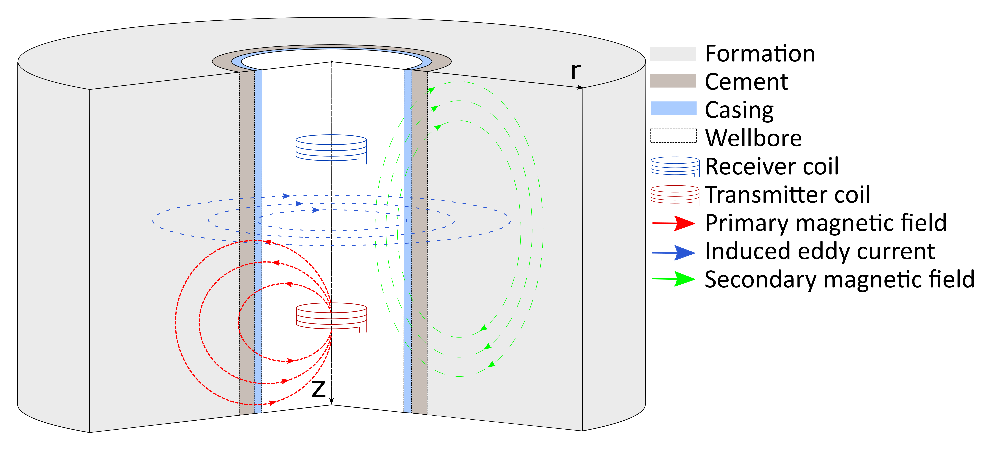
\includegraphics[scale=1.0]{Borehole_big.eps}
\vskip2pt
\caption{Schematic representation of an idealized geoelectric system. }
\label{geoelectricmodel}
\end{figure}
Key model assumptions are:
\begin{itemize}

\item The system consists of 4 concentric cylinders -- wellbore, casing, cement and formation -- with constant electrical properties along the $z$-axis,
\item All layers are isotropic and homogeneous,
\item Wellbore is an infinite column of liquid and its axis coincides with the common axis of all cylinders,
\item Coil axes coincide with the wellbore axis, and
\item Compared with the tool size, coils are small and can be approximated by point dipoles.
\end{itemize}

Signals are obtained from a solution of the Helmholtz equation in cylindrical coordinates ($r$, $\varphi$, $z$):
\begin{equation}
\frac{1}{r} \frac{\partial}{\partial r} \Big( r \frac{\partial A_z}{\partial r} \Big) + \frac{1}{r^2}  \frac{\partial^2 A_z}{\partial \varphi^2} + \frac{\partial^2 A_z}{\partial z^2} + k^2 A_z = 0
\end{equation}

\begin{equation}
H_z = k^2 A_z + \frac{\partial^2 A_z}{\partial z^2}; \;  H_r = \frac{\partial^2 A_z}{\partial r\partial z}; \; E_\varphi = i \omega \mu \frac{\partial A_z}{\partial r}.
\end{equation}

\begin{equation}
{k_m}^2 =  - i \omega \mu_m (\sigma_m - i \omega \epsilon_m)
\end{equation}
where $A_z$  is the vector potential; $\omega$ is the angular frequency; $\mu_m = \mu_{r,m} \mu_0$, the magnetic permeability ($\mu_{r,m}$ - relative, $\mu_0$ - permeability of vacuum, $m$ - the layer index); $\sigma_m$ is the electrical conductivity; and $\epsilon_m$ is the dielectric permittivity ($\epsilon_{m}=\epsilon_r \epsilon_0$, $r$ - relative, $0$ - permittivity of vacuum). Since at low frequencies the contribution of the dielectric constant is negligible, the relative permittivity of all layers is set to 1 in solving this problem.

The vector potential in the wellbore is:

\begin{equation}
A_{z, 1}(r,z) = \frac{M}{4\pi} \left( \frac{ e^{-ik_1 R}}{R} + \frac{2}{\pi} {\int_0^\infty C_1 I_0 (\lambda_1 r) \cos \lambda z \; d \lambda}\right)
\end{equation}

\begin{equation}
\lambda_m = \sqrt{\lambda^2 + i \sigma_m \mu_m  \omega }\: , \: R = \sqrt{r^2+z^2}>0
\end{equation}
Here $M$ is the magnetic moment of the coil; $\lambda$ is the separation variable; $r$ the radial distance; $z$ the axial distance; $k_1$ is the wave number corresponding to the borehole; and $C_1$ is a constant that carries information about the borehole environment and is obtained from the boundary conditions.

The measured signals are the phase, $\varphi_m$, and the amplitude, $A_m$, of the electromotive force induced by the magnetic field in the receiving coil:

\begin{equation}
a = Re(H_{z}) , \hspace{0.5cm}
b = Im(H_{z})
\end{equation}



\begin{equation}
\varphi_m = \arctan \left( \frac{b}{a} \right), \hspace{0.5cm}
A_m =  {\sqrt{a^2+b^2}}
\label{varphi}
\end{equation}

The electrical properties of the media are listed in Table ~\ref{geoelectric_table}. Wellbore, which passes through a carbonate formation, is filled with a fresh water-based mud. The well is cased with a fiberglass casing. The magnetic permeability of cement depends on the concentration of iron powder in it.

\begin{table}
\begin{center}


\begin{tabular}{|c|c|c|c|c|}
\hline
\textbf{Parameter} & \textbf{Wellbore} & \textbf{Fiberglass casing}& \textbf{Cement} & \textbf{Formation} \\
\hline
Radius, $m$             & 0.07 & 0.10 & 0.15 &  \\
Resistivity, $\Omega\cdot m$    & 2 & $10^8$ & 100 & 50 \\
Magnetic permeability & 1 & 1 & 1, 1.25, 1.5, 2 & 1  \\
\hline

\end{tabular}
\caption{Geoelectric model parameters.}
\label{geoelectric_table}
\end{center}
\end{table}

\section{Results}

\begin{figure}[ht!]
\begin{minipage}{0.5\linewidth}
\center{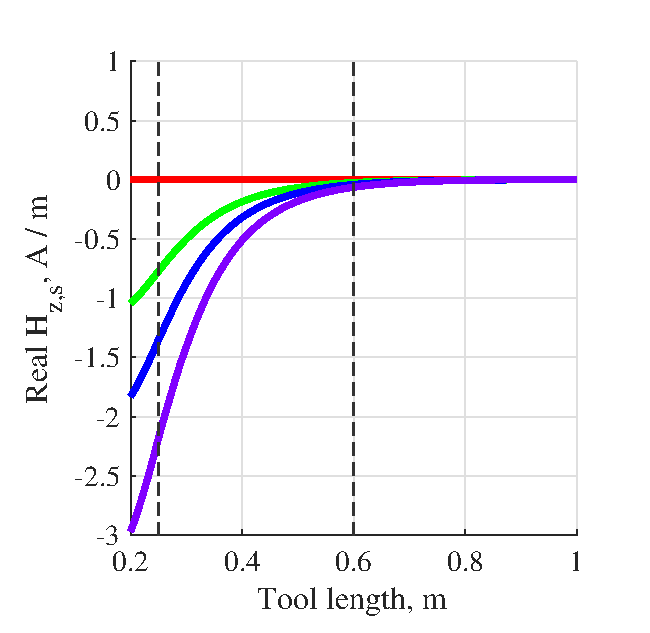
\includegraphics[clip,width=1\linewidth]{H_re_mu.eps} \\ a)}
\end{minipage}
\hfill
\begin{minipage}{0.5\linewidth}
\center{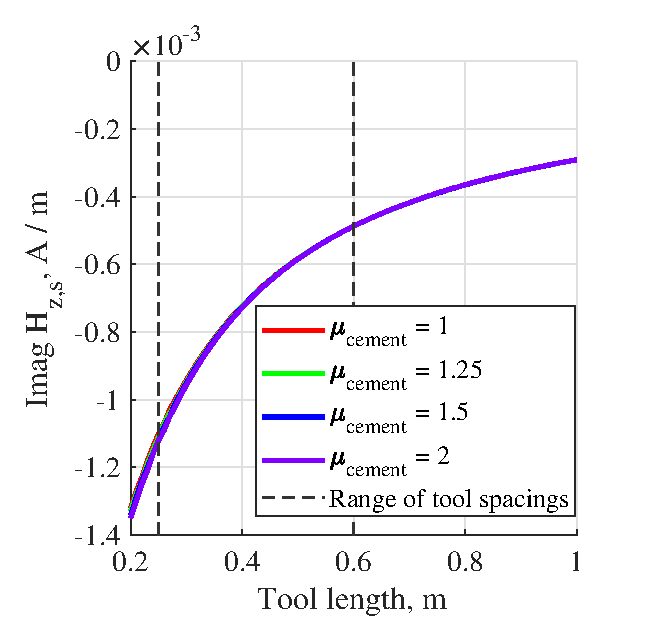
\includegraphics[clip,width=1\linewidth]{H_im_mu.eps} \\ b)}
\end{minipage}

\caption{Effect of magnetic permeability of cement on magnetic field at frequency = 1 kHz: a) Tool length vs. real part of secondary field, $H_{z,s}$. b) Tool length vs. imaginary part of $H_{z,s}$. }
\label{magfields}
\end{figure}


\begin{figure}[ht!]
\begin{minipage}{0.5\linewidth}
\center{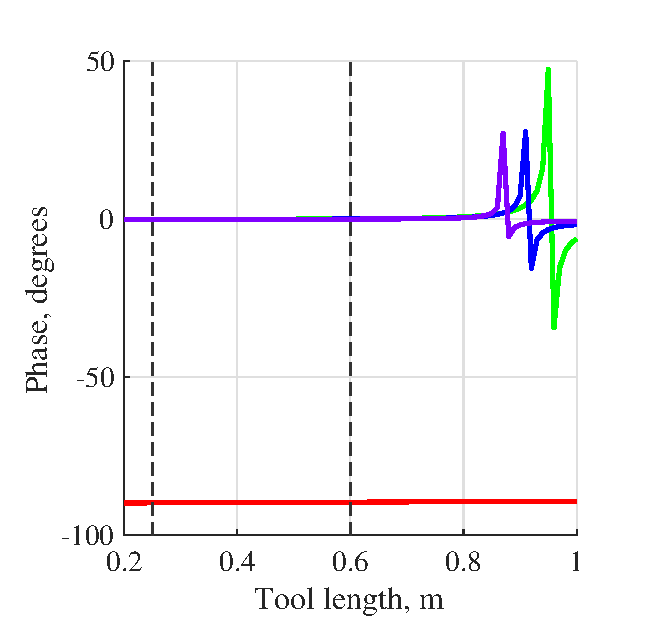
\includegraphics[clip,width=1\linewidth]{phase_mu.eps} \\ a)}
\end{minipage}
\hfill
\begin{minipage}{0.5\linewidth}
\center{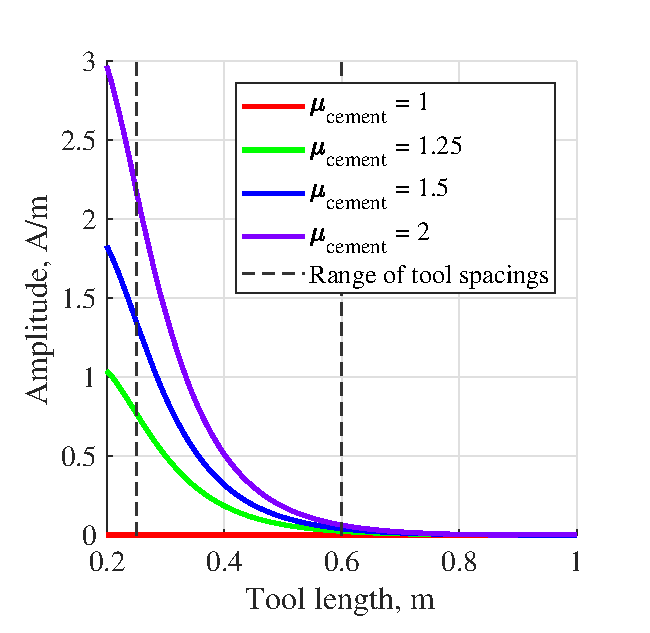
\includegraphics[clip,width=1\linewidth]{ampl_mu.eps} \\ b)}
\end{minipage}
\caption{Effect of magnetic permeability of cement on induction logging signals at frequency = 1 kHz: a) Phase vs. tool length. b) Amplitude vs. tool length. }
\label{signals}\

\end{figure}

To understand the signals that should be used to extract magnetic properties of the medium, it is necessary to analyze the magnetic field itself, as well as the response of the media under study. We assume that the tool is properly calibrated, i.e., primary magnetic field has been excluded from the measurements. Fig.~\ref{magfields} shows that the real part of secondary field, $H_{z,s}$, is three orders of magnitude stronger than the imaginary part. Smaller spacings between coils enhance detection of magnetic permeability of cement and  the distance between the coils ought to be 25 -- 60 cm (dashed line) to optimize this detection.


We have modeled the magnetic tool responses to changes of the drilling fluid resistivity, formation resistivity, cement hardening and magnetic permeability of the cement (amount of magnetic particles). The amount of magnetic powder in the cement has a strong influence on real part of the secondary field, $H_{z,s}$, i.e., useful information about cement integrity can be extracted from it. Curves for the different resistivities of cement, mud and formation overlap. Changes in the frequency of the transmitter coil in the lower part of the kHz range do not significantly affect the real part of $H_{z,s}$. At the same time, changes in the frequency affect the imaginary part of $H_{z,s}$ more strongly in the upper kHz range. {With increasing frequency, the amplitude of the imaginary part of $H_{z,s}$ grows and becomes of the same order as that of the real part.} Therefore, we propose to use the frequencies ranging from 0.1 to 10 kHz, typical of magnetic susceptibility logging. Typical pattern of $H_{z,s}$ vs. tool length is presented in Fig.~\ref{magfields}.

Fig.~\ref{signals} shows that the signal amplitude is suitable for extracting magnetic properties of cement. Simulation results presented in Fig.~\ref{magfields} and Eq.~(\ref{varphi}) support this conclusion. The signal amplitude is insensitive to cement resistivity, i.e., cement rheology in the frequency range from 0.1 to 10 kHz. Signal simulations for different configurations of borehole geometry show that the singularities of the signal phase are caused by the magnetized cement and its distance from the measurement point.

\begin{figure}[ht!]
\begin{minipage}{0.5\linewidth}
\center{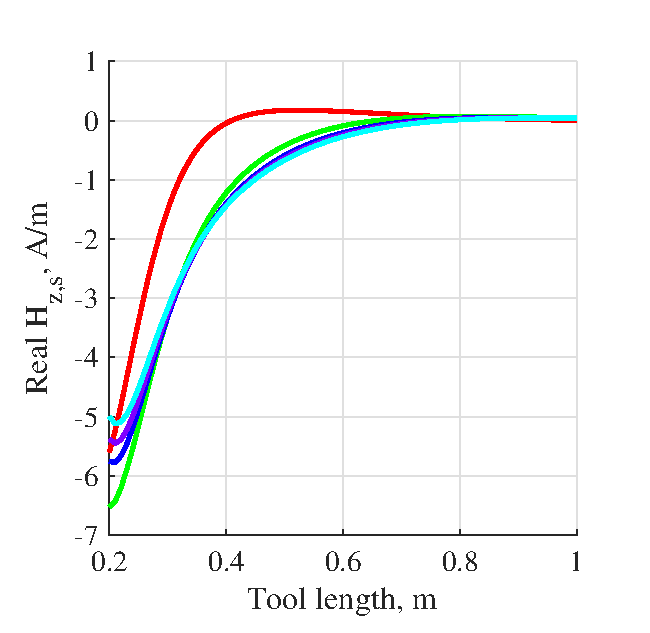
\includegraphics[clip,width=1\linewidth]{cem_hd_re.eps} \\ a)}
\end{minipage}
\hfill
\begin{minipage}{0.5\linewidth}
\center{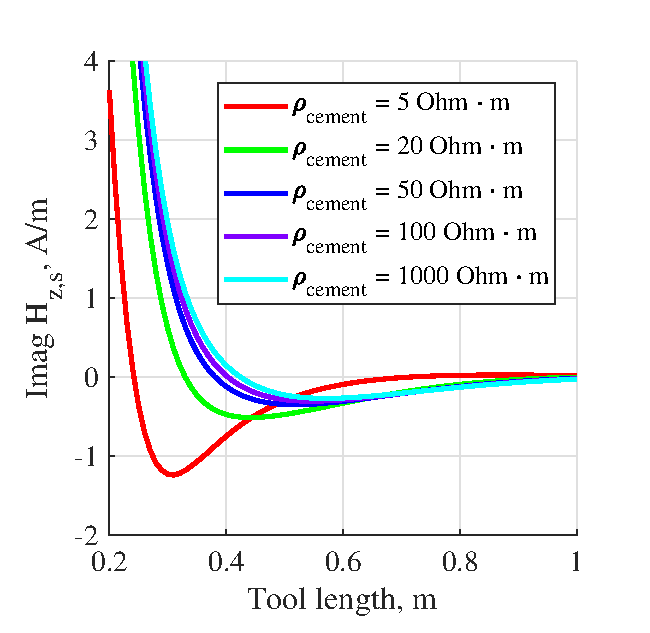
\includegraphics[clip,width=1\linewidth]{cem_hd_im.eps} \\ b)}
\end{minipage}
\caption{ Intensity of a) real and b) imaginary part of $H_{z,s}$ vs. tool length at frequency = 200 MHz. Different state of the cement is considered: the harder the cement the higher the resistivity.}
\label{cement_hard}\

\end{figure}

\begin{figure}[ht!]
\center{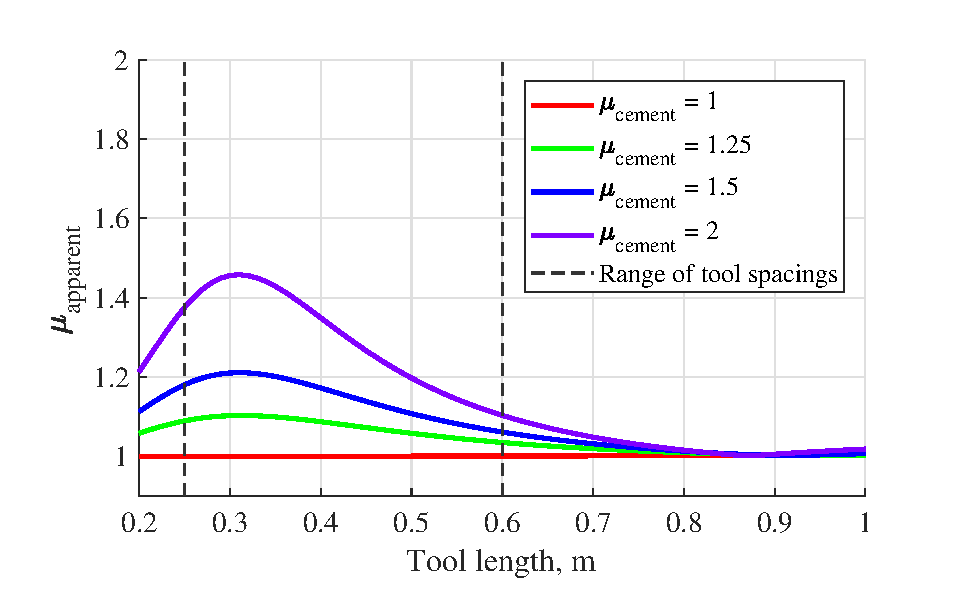
\includegraphics[clip,width=0.8\linewidth]{mu_apparent_big.eps}}
\caption{ Apparent magnetic permeability vs. tool length at frequency = 1 kHz. }
\label{mu_apparent}\

\end{figure}

\subsection{Sensing solidification of concrete.}
It is known that the electrical resistance of cement depends on the degree of its solidification. The electrical resistivity of cement grows as it solidifies  \citep{Sallehi2015}. The rate of resistivity growth depends on water fraction in the cement paste or foam, water conductivity, and other parameters. These questions go beyond our research objectives. It is important for us to know only the aggregate state of cement.  For simplicity, it can be said that the cement paste has an electrical resistance below 5 Ohm$\cdot$m. Cement with $>$ 50 Ohm$\cdot$m resistivity might be considered as solid. It reaches this resistance in several hours and with time the resistance slowly grows \citep{Osterminski2012}. How can one detect a relatively conductive cement-filled annulus behind a non-conducting casing? Methods for measuring DC resistance are not suitable for this task. Fiberglass casing is a resistor and current will not flow through it. To measure cement resistance, one can use a high frequency induction method. The high frequency EM field weakly damps in the insulator and penetrates into the cement annulus. The best results can be achieved by pressing the tool against the wall of the wellbore. This is necessary to minimize signal losses in drilling mud.

Imaginary part of the magnetic field intensity is influenced by the change of cement resistivity, see Fig.~\ref{cement_hard}. This figure shows the imaginary part of the secondary magnetic field versus distance between the transmitter and receiver. The source is a point dipole oscillating at the frequency 200 MHz. The geometric and electric parameters are listed in Table \ref{geoelectric_table}. The relative magnetic permeability of the cement is 1.5. In this case, a two-coil tool and a three-coil tool can be used. It is recommended to use tools with the separation between coils ranging from 0.3 to 0.4 m. We conclude that soft cement can be detected at high frequency.




\subsection{Apparent magnetic permeability.}

{Our calculation of the apparent magnetic permeability is based on the assumption of homogeneity of the medium. Change of the real part of magnetic field is proportional to the change of magnetic permeability of the medium. It is worth describing the calculation of geometrical and demagnetization coefficients, as they determine the conditions of measurements. In a homogeneous environment, these coefficients are expressed as \citep{Saraev2004}:}
\begin{equation}
G \ae' = \frac{\xi_{z,s}+\xi_{z,p}}{\xi_{z,p}}, \quad   \ae' = \frac{\ae'}{(1+N\ae)}
\label{gandn}
\end{equation}
{Here $\ae'$ is the apparent magnetic susceptibility, ($\mu_{apparent} = 1+\ae$); $G$, the geometrical coefficient; $\xi$, the electromotive force; $N$, the demagnetization factor; and $p$ and $s$ denote the primary and secondary field indices. The imaginary part in the preferred frequency range in Fig.~\ref{magfields} is negligible when compared with the real part. In this case, the amplitude is equal to the modulus of the real part of the magnetic field, see Eq. (\ref{varphi}). Magnetic susceptibility can be expressed as:}
\begin{equation}
\frac{\ae}{1+N \ae} = \frac{\xi_{z,s}+\xi_{z,p}}{G \xi_{z,p}}, \quad   \xi = i\omega\mu\sigma H_{z}
\label{apparent_eq}
\end{equation}
Here $\ae$ is the magnetic susceptibility of the medium. From general solution of the boundary problem, and in accordance with Eq.~(\ref{gandn}), we obtain the geometrical and demagnetization coefficients:
\begin{equation}
G  = \lim_{\ae\to 0} \frac{\xi_{z,s}+\xi_{z,p}}{\ae\xi_{z,p}}, \quad N = \frac{G\xi_{z,p}}{\xi_{z,s}+\xi_{z,p}} - \frac{1}{\ae}
\label{geometric}
\end{equation}
These coefficients can be calculated from experimental data by solving a system of linear equations:
\begin{equation}
\frac{\xi_{z,s}+\xi_{z,p}}{\ae\xi_{z,p}}(1+N\ae_i)=G\ae_i,\quad i = 1,2,...
\label{lineq}
\end{equation}
{Here $i$ is the subscript of the medium with the magnetic susceptibility $\ae_i$. Apparent magnetic permeability, see Fig.~\ref{mu_apparent}, differs from the actual permeability of magnetic cement because only a part of the medium is magnetic. The apparent magnetic permeability has been calculated from the signal amplitude in Fig.~\ref{signals} b. Finally, short tools are more sensitive to the magnetic properties of cement.}

\subsection{The analytic solution and the finite element method.}

\begin{figure}[ht!]
\begin{minipage}{0.5\linewidth}
\center{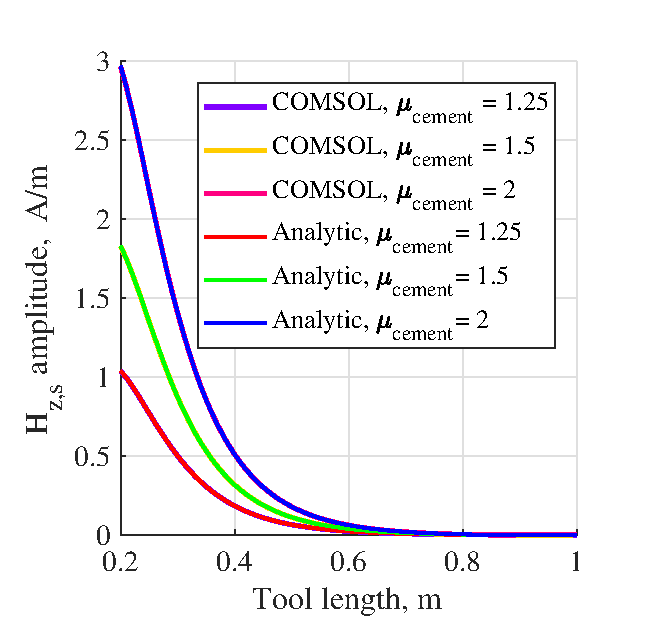
\includegraphics[clip,width=1\linewidth]{comsol_compar_ampl.eps} \\ a)}
\end{minipage}
\hfill
\begin{minipage}{0.4\linewidth}
% Wellbore 7, casing 3 different cement thickness
\center{\includegraphics[clip,width=1\linewidth]{Magnetic_dipole.eps} \\ b)}
\end{minipage}
\caption{a) Comparison of useful signal amplitude computed using COMSOL and analytic solution and b) Propagation of the magnetic field generated by a point dipole source in the wellbore at the frequency of 1 kHz (COMSOL). }
\label{comsol_compare}\

\end{figure}

\begin{figure}[ht!]
\begin{minipage}[h]{0.23\linewidth}
\center{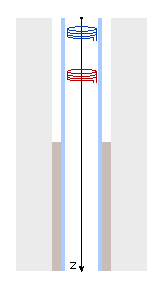
\includegraphics[width=1\linewidth]{Borehole_cementlift.eps}} a) \\
\end{minipage}
\hfill
\begin{minipage}[h]{0.26\linewidth}
\center{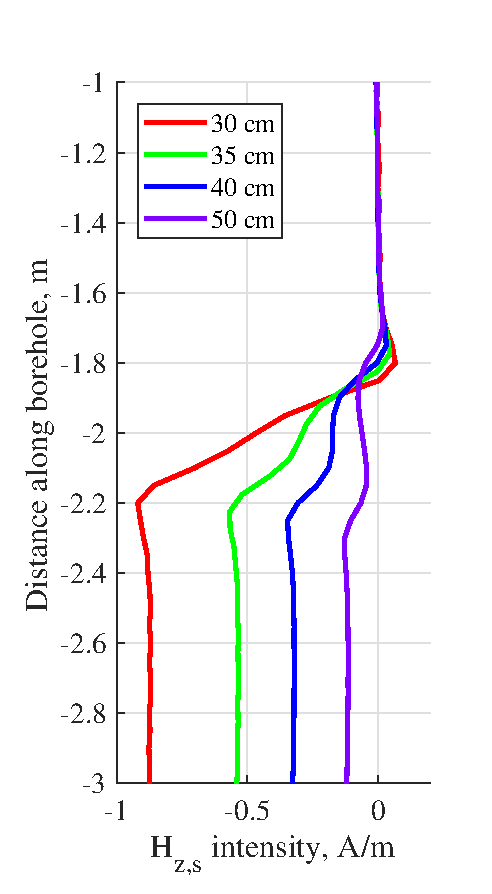
\includegraphics[width=1\linewidth]{logging_cemlift.eps}} \\ b)
\end{minipage}
\hfill
\begin{minipage}[h]{0.23\linewidth}
\center{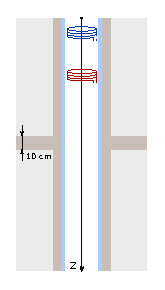
\includegraphics[width=1\linewidth]{Borehole_crack.eps}} c) \\
\end{minipage}
\hfill
\begin{minipage}[h]{0.26\linewidth}
\center{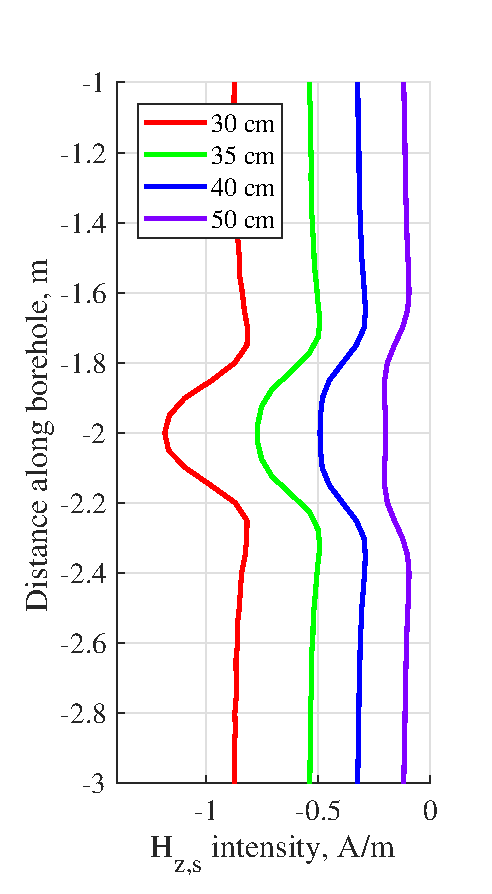
\includegraphics[width=1\linewidth]{logging_crack.eps}} d) \\
\end{minipage}
\caption{a) The model of incomplete lift of cement, b)
logging signals at the frequency = 1 kHz cross a cement lift c) the model crack filled with magnetic cement, d) logging signals at the frequency = 1 kHz cross a crack filled with magnetic cement, different tool lengths are considered.}
\label{liftandcrack}
\end{figure}

\begin{figure}[ht!]
\begin{minipage}[h]{0.23\linewidth}
\center{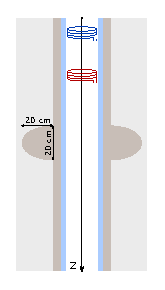
\includegraphics[width=1\linewidth]{Borehole_cavity.eps}} a) \\
\end{minipage}
\hfill
\begin{minipage}[h]{0.26\linewidth}
\center{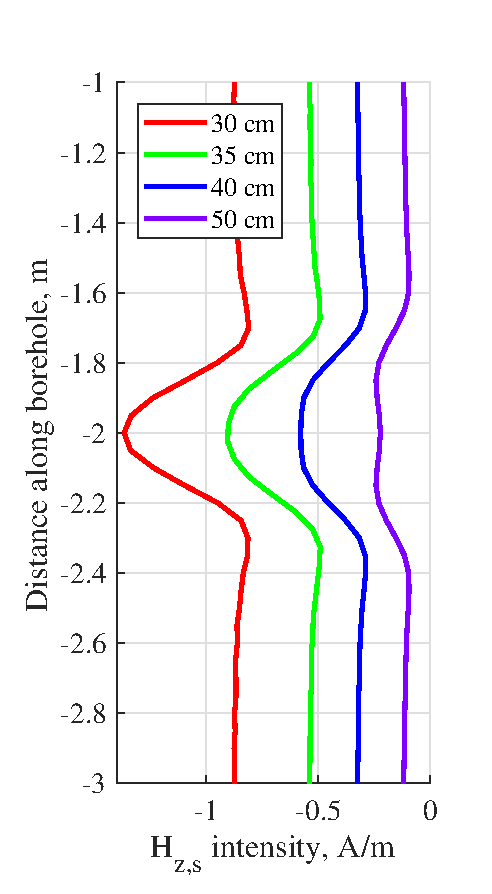
\includegraphics[width=1\linewidth]{logging_cavity.eps}} \\ b)
\end{minipage}
\hfill
\begin{minipage}[h]{0.23\linewidth}
\center{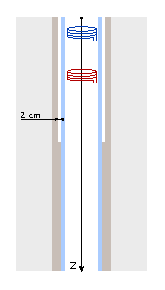
\includegraphics[width=1\linewidth]{Borehole_debonding.eps}} c) \\
\end{minipage}
\hfill
\begin{minipage}[h]{0.26\linewidth}
\center{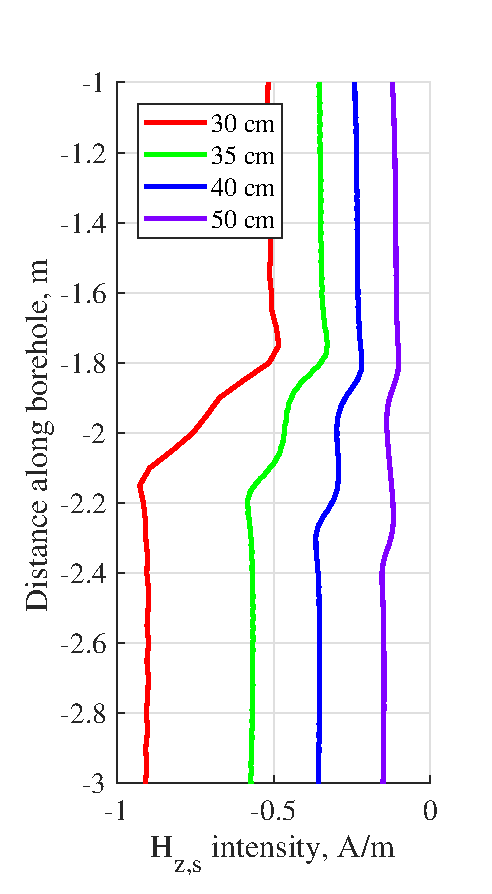
\includegraphics[width=1\linewidth]{logging_debond.eps}} d) \\
\end{minipage}
\caption{a) The model of a cavity filled with a cement, b) Logging signals at the frequency = 1 kHz cross a cavity filled with cement c) the model of a cement with 2 cm debonding, d) logging signals at the frequency = 1 kHz cross a debonding area.}
\label{cavityanddebond}
\end{figure}

\begin{figure}[ht!]
\begin{minipage}[h]{0.26\linewidth}
\center{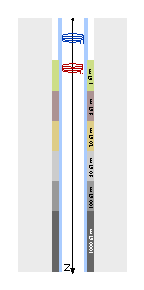
\includegraphics[width=1\linewidth]{cement_solid_model.eps}} a) \\
\end{minipage}
\hfill
\begin{minipage}[h]{0.34\linewidth}
\center{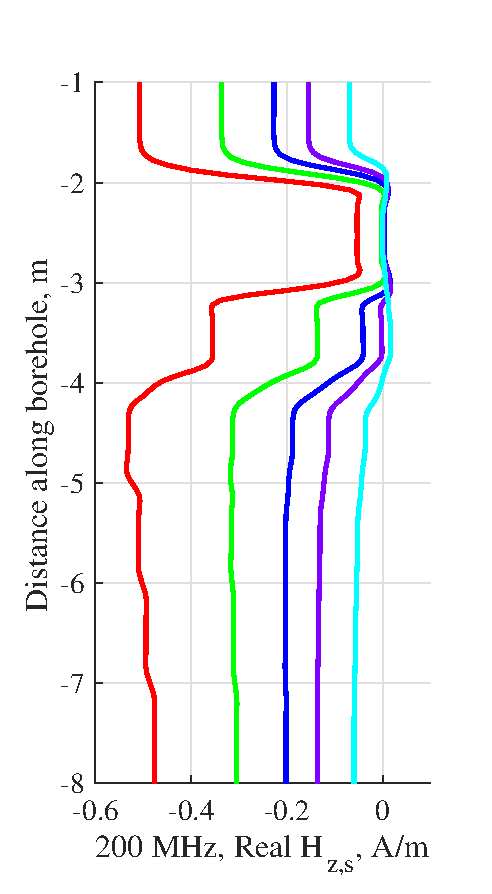
\includegraphics[width=1\linewidth]{cement_solid_logg_Hre.eps}} \\ b)
\end{minipage}
\hfill
\begin{minipage}[h]{0.34\linewidth}
\center{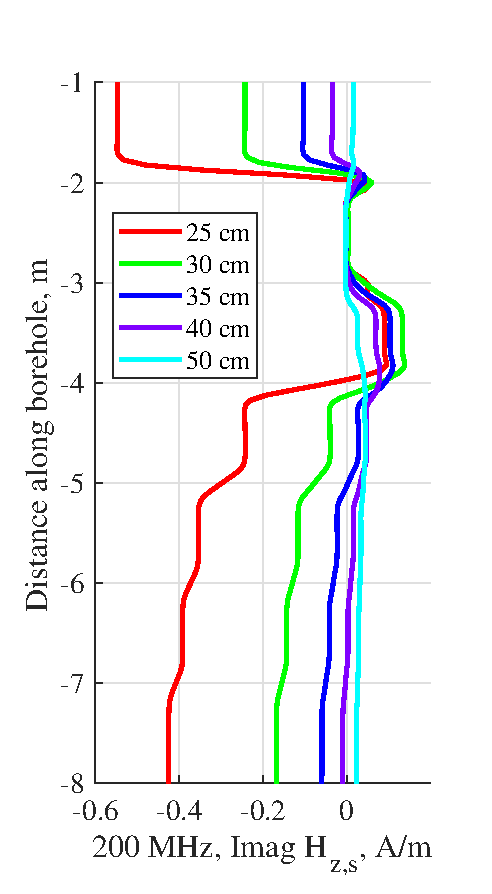
\includegraphics[width=1\linewidth]{cement_solid_logg_Him.eps}} c) \\
\end{minipage}
\hfill
\caption{a) The wellbore model with different resistivities of the cement (different solidification states) and induction logging signals at the frequency = 200 MHz for b) real and c) imaginary part of $H_{z,s}$. Different tool lengths are considered.}
\label{logging_cement_solid}
\end{figure}

\begin{figure}[ht!]
\begin{minipage}[h]{0.26\linewidth}
\center{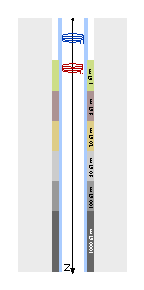
\includegraphics[clip,width=1\linewidth]{cement_solid_model.eps}} a) \\
\end{minipage}
\hfill
\begin{minipage}[h]{0.34\linewidth}
\center{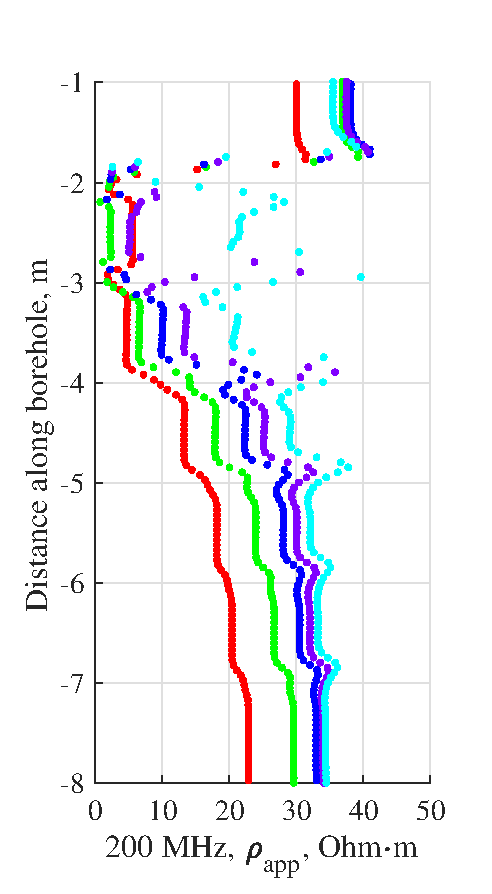
\includegraphics[clip,width=1\linewidth]{cement_solid_logg_rapp_phs.eps}} \\ b)
\end{minipage}
\hfill
\begin{minipage}[h]{0.34\linewidth}
\center{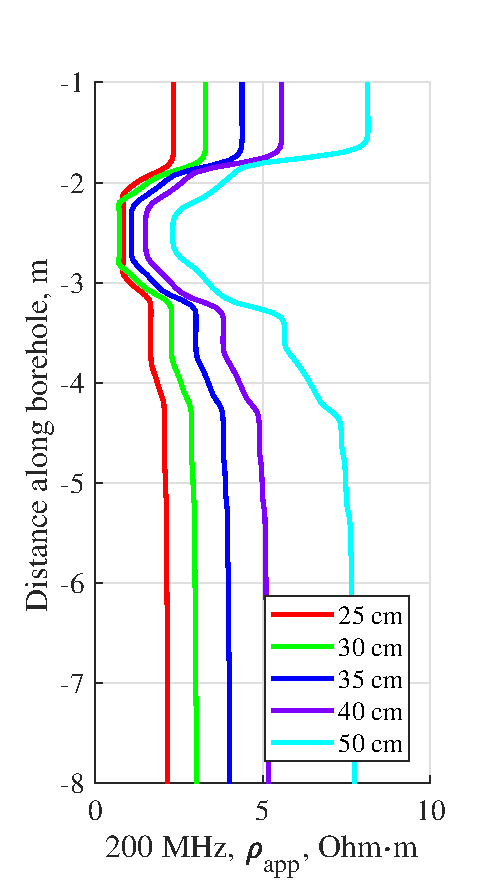
\includegraphics[clip,width=1\linewidth]{cement_solid_logg_rapp.eps}} c) \\
\end{minipage}
\hfill
\caption{a) The wellbore model with different resistivities of the cement (different solidification states) and apparent resistivity at the frequency = 200 MHz calculated from b) signal phase and b) amplitude. Different tool lengths are considered. }
\label{logging_cement_solid_app}
\end{figure}

COMSOL software calculations and analytic solutions are identical, see Fig. ~\ref{comsol_compare}a. We consider a point magnetic dipole, oscillating at a frequency of 1 kHz. The dipole is located at the origin, the length of the well is 3 m, the diameter of the model is 3 m, and the geometric and electrical parameters of the model are from Table ~\ref{geoelectric_table}.  {The nonuniform mesh parameters used in the modeling are: the maximum element size $=1$ cm and the minimum one $=8\cdot10^{-5}$ m. Maxwell's equations are solved in the frequency domain and the number of degrees of freedom is 1199956. The external boundary is assumed to be a magnetic and electric insulator. Due to the short length of the probes relative to the model size, the influence of the external boundary can be neglected.} To obtain the secondary magnetic field, the simulations were carried out in two environments, air and the medium under study. The response in air was subtracted, i.e., the tool response was calibrated.
The signals were calculated using equations ~(\ref{varphi}). The signals computed with the finite element method are less smooth than those from the analytical calculations. The magnetic field strength scale is amplified in Fig. ~\ref{comsol_compare}b to improve visualization of the field propagation. Relative to a non-magnetic medium, a magnetic cement with $\mu$=2 is practically a ``magnetic conductor''.

\begin{figure}[ht!]
\begin{minipage}{0.50\linewidth}
\center{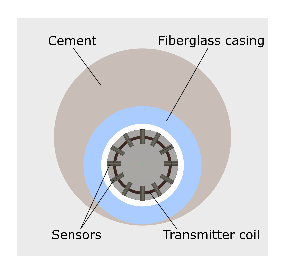
\includegraphics[clip,width=1\linewidth]{tool_face_ecctr.eps} \\}
\end{minipage}
\hfill
\begin{minipage}{0.50\linewidth}
% Cement lift
\center{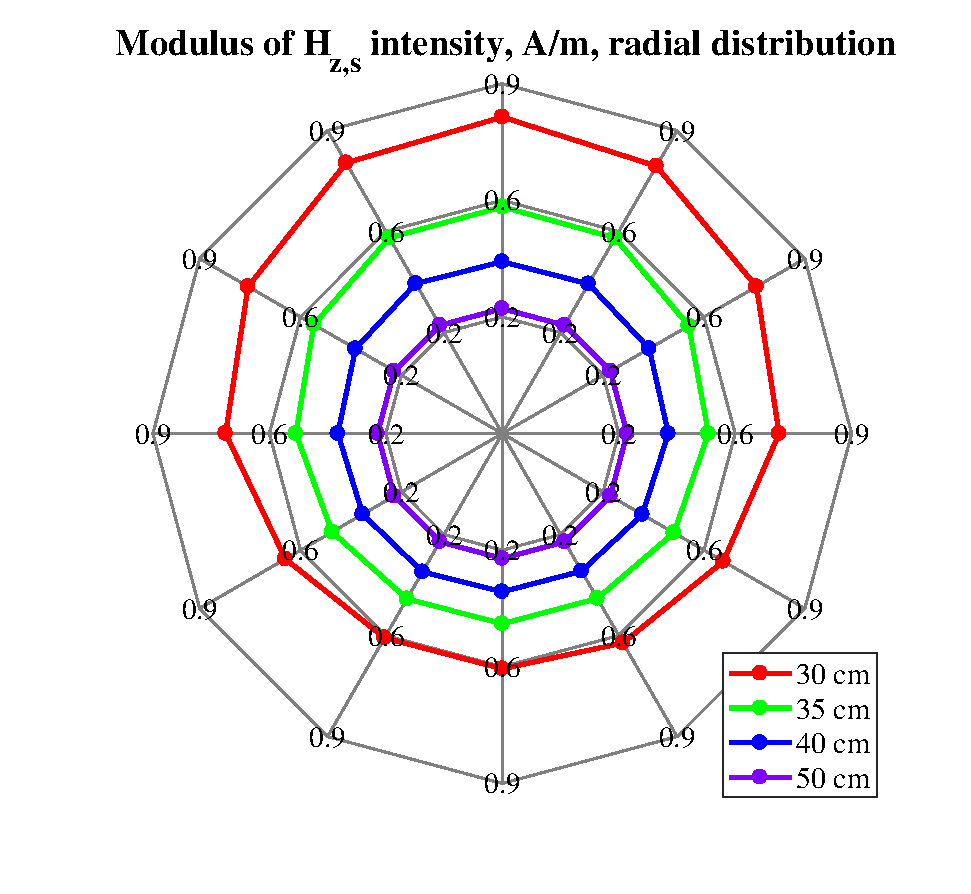
\includegraphics[clip,width=1\linewidth]{cement_ecctr.eps} \\}
\end{minipage}
\caption{Facet of eccentric wellbore filled with magnetic cement. The signal frequency = 1 kHz. }
\label{facet_ecctr_cement}\
\end{figure}

\begin{figure}[ht!]
\begin{minipage}{0.50\linewidth}
\center{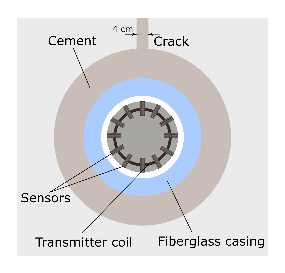
\includegraphics[clip,width=1\linewidth]{facet_crack_model.eps} \\}
\end{minipage}
\hfill
\begin{minipage}{0.50\linewidth}
% Cement lift
\center{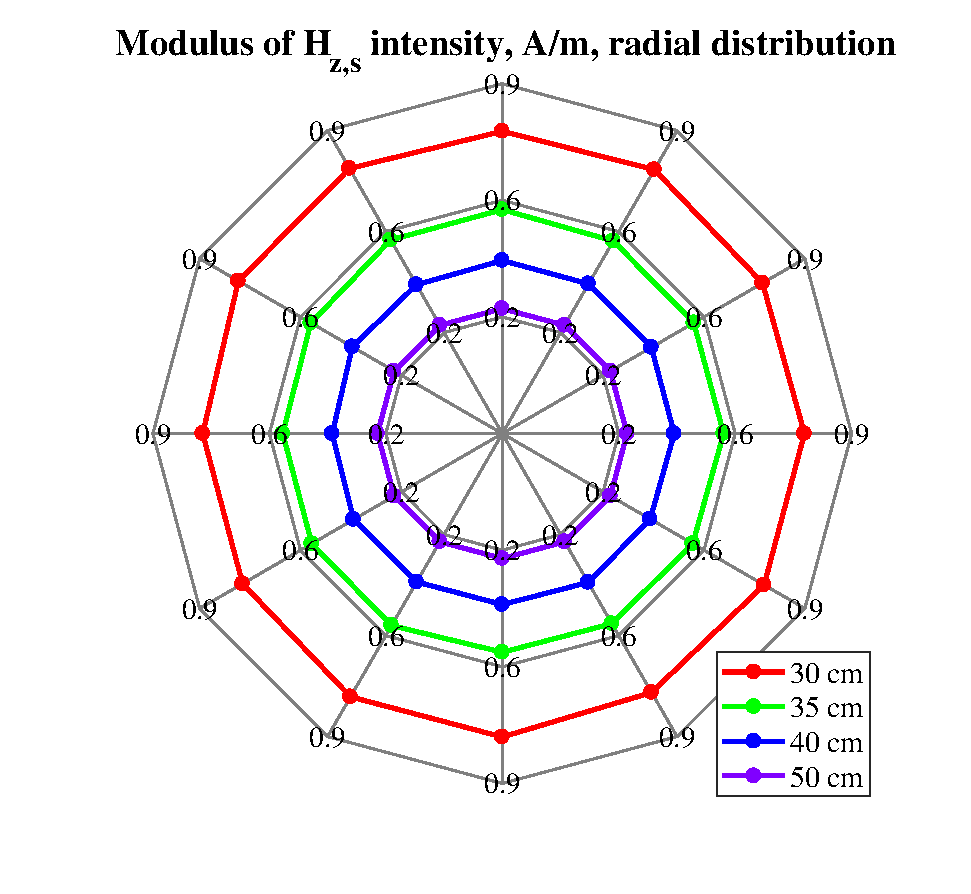
\includegraphics[clip,width=1\linewidth]{facet_crack.eps} \\}
\end{minipage}
\caption{Facet of wellbore and crack filled with magnetic cement. The signal frequency = 1 kHz. }
\label{facet_crack}\

\end{figure}

\subsection{Logging signal modeling.}

To test the technology being developed, we perform numerical testing of magnetic logging for five scenarios: (1) incomplete lift of cement, (2) cavity, (3) crack filled with magnetic cement, (4) 2 cm cement debonding, and (5) progress of cement solidification along borehole. The 2D axisymmetric simulations were performed using the AC/DC module in COMSOL. The source of electromagnetic waves is a point dipole with the magnetic moment = 1 $A/m$.  The dipole oscillates at the frequency of 1 kHz for scenarios 1 - 4. The magnetic moment is 0.1 $A/m${ and the frequency 200 MHz for the 5th scenario}. Probes with the lengths of 30, 35, 40 and 50 cm pass through a wellbore interval with inhomogeneities. The geometric and electric parameters are listed in Table \ref{geoelectric_table}. The relative magnetic permeability of the cement is 1.5. Response in the air was subtracted. {For the 5th scenario, six different cement resistivities were used to depict its solidification:  1, 5, 20, 50, 100 and 1000 Ohm$\cdot$m. In this case, cement tubes 1 meter high lie on top of each other, and the space above 1 Ohm$\cdot$ m tube is filled with air. For cement solidification state, an additional 25 cm long tool is considered, because at high frequencies the skin depth, $ \Big(  \delta = \sqrt{\frac{2}{\sigma\mu \omega}}$, $\sigma$ being the electrical conductivity$\Big)$ significantly decreases.

Figs. \ref{liftandcrack} a and b} show that incomplete rise of cement can be determined by an abrupt decrease of amplitude of the secondary magnetic field. Figs. \ref{liftandcrack} c, d and  Fig. \ref{cavityanddebond} a, b demonstrate that the proposed tool is capable of detecting cement inhomogeneities and it is more sensitive to the near wellbore region. The shape and intensity of magnetic logging curves are determined by the shapes of heterogeneities filled with cement. Cement adjacent to the well casing generates the strongest tool response. Absence of cement results in a sharp decrease of magnitude of the secondary magnetic field observed in Fig. \ref{cavityanddebond} c, d.

When logging at 200 MHz, see Fig. \ref{logging_cement_solid} and Fig. \ref{logging_cement_solid_app}, one can observe a stair-step change of the real and imaginary part of $H_{z,s}$. It is important to note that in this particular case, magnitudes of the imaginary and real parts of $H_{z,s}$ are very close and the stair-step changes are opposite for both components. To calculate the apparent electrical resistivity from signal amplitude, a homogeneous medium approximation is used. The apparent resistivity calculation algorithm was described in \citep{Eltsov2013}. {There are many ways of transforming signals into apparent resistivities, e.g., the pallet method, optimization methods, and asymptotic formul\ae. To convert signals into apparent resistivities, the Newton method was chosen for efficiency. To ensure convergence in a small number of iterations using this method, a good initial guess is necessary. The exact formul\ae~for calculating induction logging signals, Eq. (\ref{varphi}), have been transformed and a good initial guess has been constructed. The apparent resistivity calculation algorithm used here is accurate to at least six significant digits.}  Fig.~\ref{logging_cement_solid_app} shows that we can easily distinguish a ``liquid'' cement (1 - 5 Ohm$\cdot$ m) from a ``solidified'' cement (50 Ohm$\cdot$ m and more). It is impossible to distinguish a 50 Ohm$\cdot$m layer from a 100 Ohm$\cdot$m one, but we can observe a trend of solidification. Short tools are more sensitive to the wellbore and measure the lowest resistivities. Longer tools better sense the near wellbore space. Due to the special nature of the electromagnetic field and model complexity, the electrical resistances calculated from the phase, Fig.~\ref{logging_cement_solid_app} b, and amplitude, Fig.~\ref{logging_cement_solid_app} c, differ significantly. For better display, Fig.~\ref{logging_cement_solid_app} b is plotted as dots, because the boundary-related singularities in the resistivity log obtained from the signal phase obscure the tool responses. However, compared with amplitude, phase is more sensitive to cement solidification state. The effect of surrounding layers is more significant for the graph generated from amplitude.

Simulations show that the zones with insufficient cementing can be easily determined using the proposed tools and we can use the high-frequency induction tool to distinguish between the zones of ``solidified'' and ``liquid'' cement.

\subsection{Detection of radial inhomogeneities.}
Magnetic logging signals have been simulated to study the possibility of detection of radial inhomogeneities: (1) the eccentricity of the cement, and (2) a crack filled with the magnetic cement. The 3D simulations were performed using the AC/DC module in COMSOL. {The model is a 1.5 m long cylinder with the diameter of 1.5 m. Complete mesh consists of 1387193 domain elements, 65048 boundary elements, and 2327 edge elements. Average element quality is 0.7679.  The source of electromagnetic waves is a point dipole with magnetic moment = 1 $A/m$, oscillating at the frequency of 1 kHz in the middle of the borehole. External boundary is assumed to be a magnetic and electric insulator.}  The distances between the transmitter and receivers are 30, 35, 40 and 50 cm. As previously, the influence of the outer boundary is neglected. The magnetic field is registered by 12 sensors evenly distributed inside the casing, see Figs. \ref{facet_ecctr_cement} and  \ref{facet_crack}. The geometric and electric parameters are listed in Table \ref{geoelectric_table}. The relative magnetic permeability of the cement is 1.5. Tool response is calibrated by subtracting the system response in the air. Fig. \ref{facet_ecctr_cement} shows that an asymmetric distribution of magnetic cement can be detected by the proposed tool. Fig. \ref{facet_crack} shows that a small radial crack filled with cement is invisible to the tool. The distance to the crack is too large and the contribution to the signal from the anomaly is less than the measurement error. However, insufficient cementation near the casing can be detected with magnetic logging signals.

\section{Conclusions}
We have optimized an induction logging tool for testing integrity of a weakly magnetic cement behind a non-conductive casing. Tools with the lengths of 0.25 - 0.6 m are most sensitive to magnetic cement properties. The real part of secondary magnetic field, $H_{z,s}$, is more sensitive to magnetic cements than the imaginary part. The most suitable frequencies for magnetic cement detection are in the range 0.1 to 10 kHz, typical of magnetic susceptibility logging. Amplitude can be used to infer integrity of magnetic cement behind casing, but to obtain information about cement rheology it is necessary to perform the high-frequency resistivity measurements. Logging at 200 MHz distinguishes solid cement from liquid and quantifies the cement solidification state. Phase at the high frequency is more sensitive to cement solidification, rather than amplitude. Cavities and cracks filled with magnetic cement are visible on the logs. The proposed tool can be used for determination of the zones of cement debonding. Casing eccentricity and radial inhomogeneities can be detected using the radially distributed sensors. Absence of cement causes a sharp decrease of magnitude of the secondary magnetic field. The magnetic logging technology proposed in this paper can be used to check cement quality in low temperature wells ($<150$  $^{\mathrm{o}}$C). The proposed method can determine poor zonal isolation and cement hardening.

\section{Acknowledgements}

Dr. Eltsov was supported by the KAUST Magnetic Sensor project.


\clearpage
\vskip -0.2in
\bibliographystyle{agu}
\bibliography{timaref}

\vskip 0.2in

\end{document}
